\chapter{Compilation - Leiserson MIT}
\section{Interpreters vs Compilers}
Interpreted languages are more versatile, but much slower.
\begin{lstlisting}
for (int i = 0; i < n; i++) {
   for (int j = 0; j < n; j++) {
      for (int k = 0; k < n; k++) {
         C[i][j] += A[i][k] +B[k][j];
      }
   }
}
\end{lstlisting}
This code executed using Clang/LLVM 5.0 takes 1156s (19m 16s) to execute, about \textbf{2x} times faster than Java and \textbf{18x} times than python


\section{Cache}
\begin{paracol}{2}
   \colfill
   \begin{lstlisting}
      for (int i = 0; i < n; i++) {
            for (int k = 0; k < n; k++) {
         for (int j = 0; j < n; j++) {
               C[i][j] += A[i][k] +B[k][j];
            }
         }
      }
   \end{lstlisting}
   \colfill

   We can change the order of the loops without changing the result, but the performance can change.

   \switchcolumn

   \begin{figure}[htbp]
      \centering
      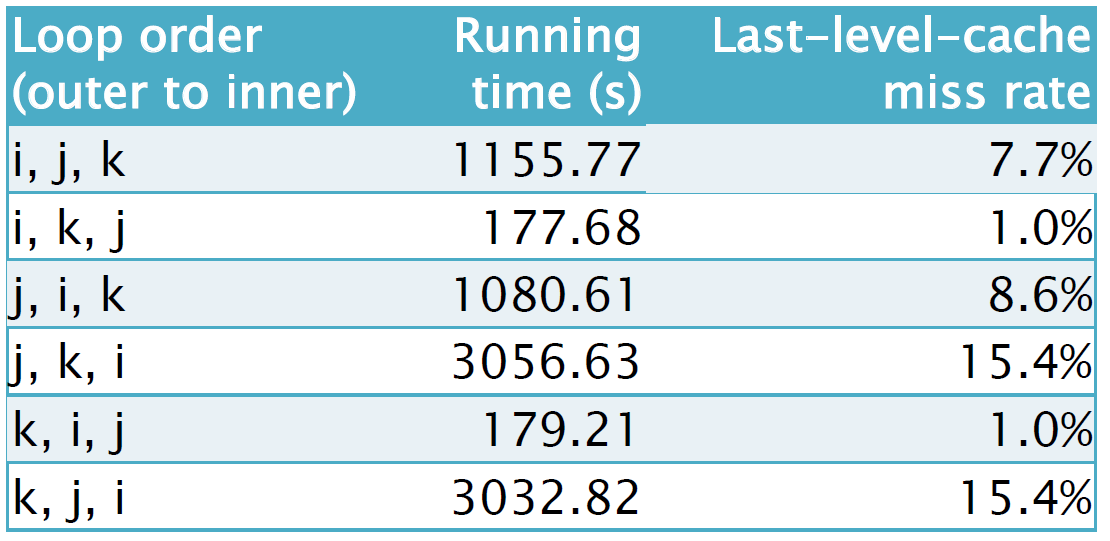
\includegraphics[width=0.9\columnwidth]{images/02/caches_looporder.png}
      \caption{Performance against loop order}
      \label{fig:02/caches_looporder}
   \end{figure}
   
\end{paracol}

As you can see, there is a huge difference in the running time of the loop depending on the loops ordering. This is due to \textbf{caching}, which consists in storing in a fast-access memory previously accessed memory lines.

\newpage
\begin{figure}[htbp]
   \centering
   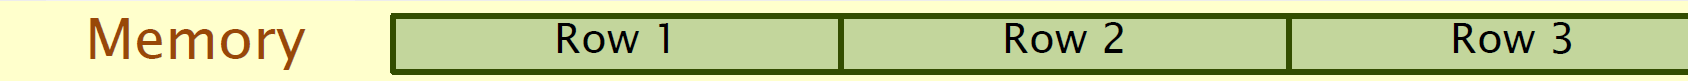
\includegraphics{images/02/rowmajor.png}
   \caption{Memory layout for matrix rows}
   \label{fig:02/rowmajor}
\end{figure}
Matrices are stored in memory in row-major order, so the first loop should iterate over the rows of the matrix, to exploit the cache.

\begin{figure}[htbp]
   \centering
   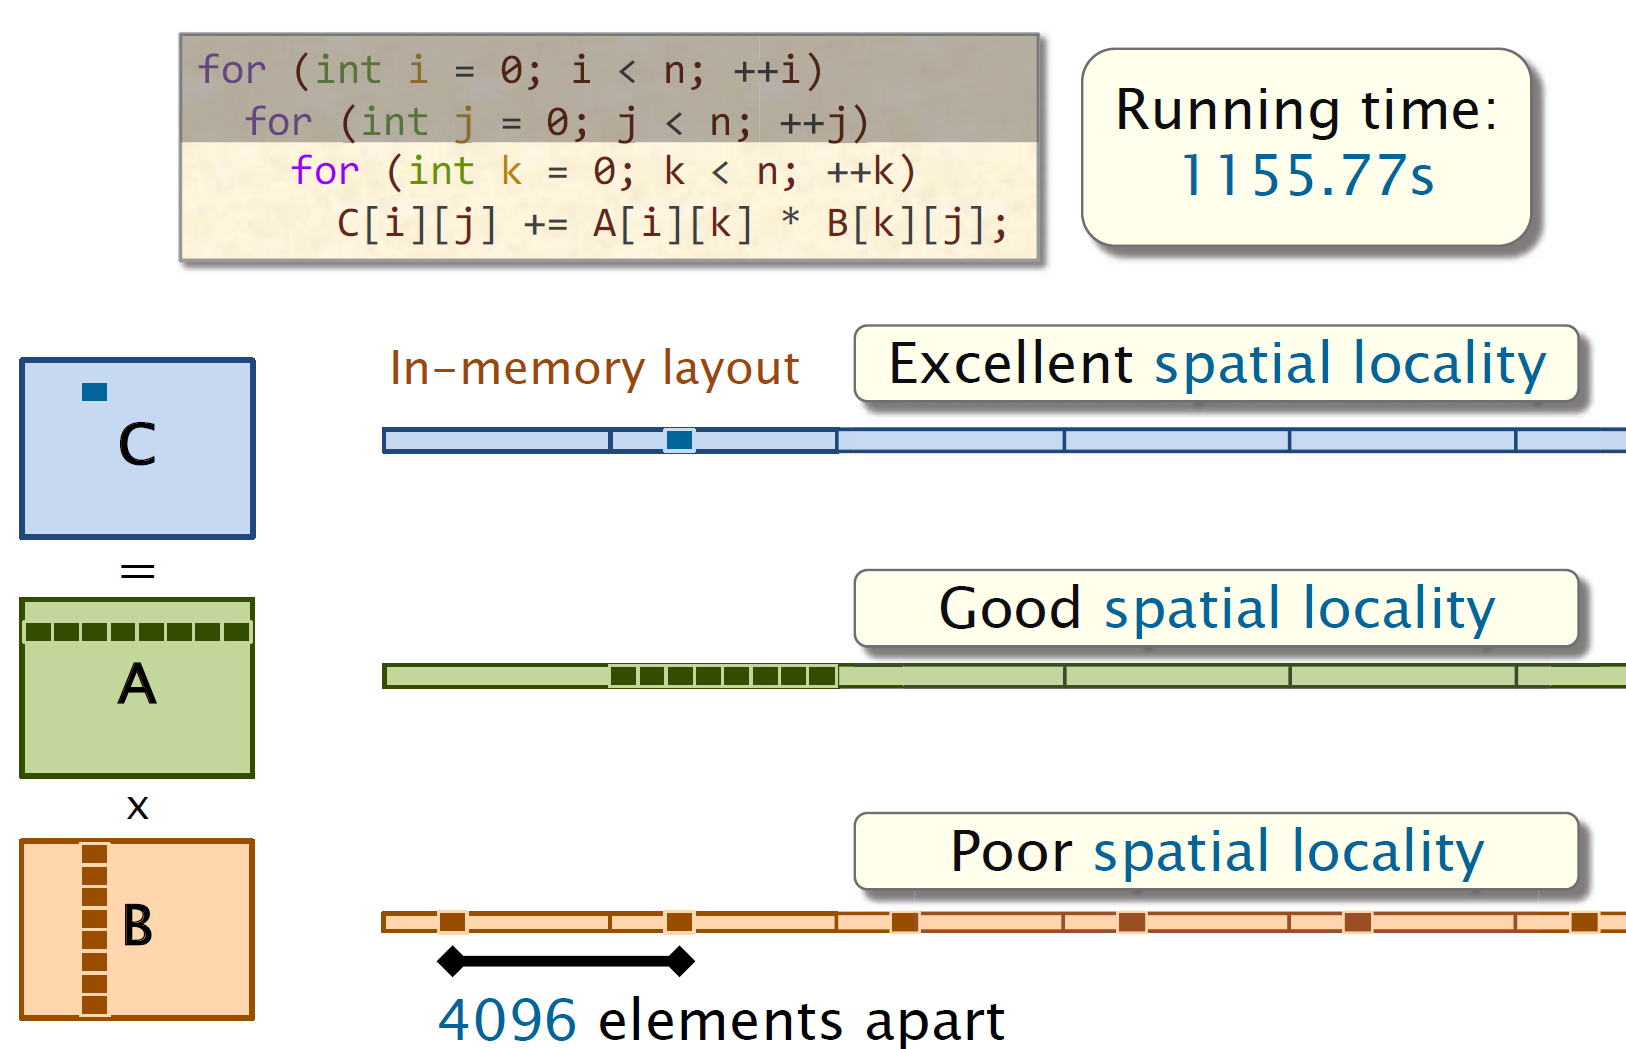
\includegraphics[width=0.49\columnwidth]{images/02/memory_layout1.png}
   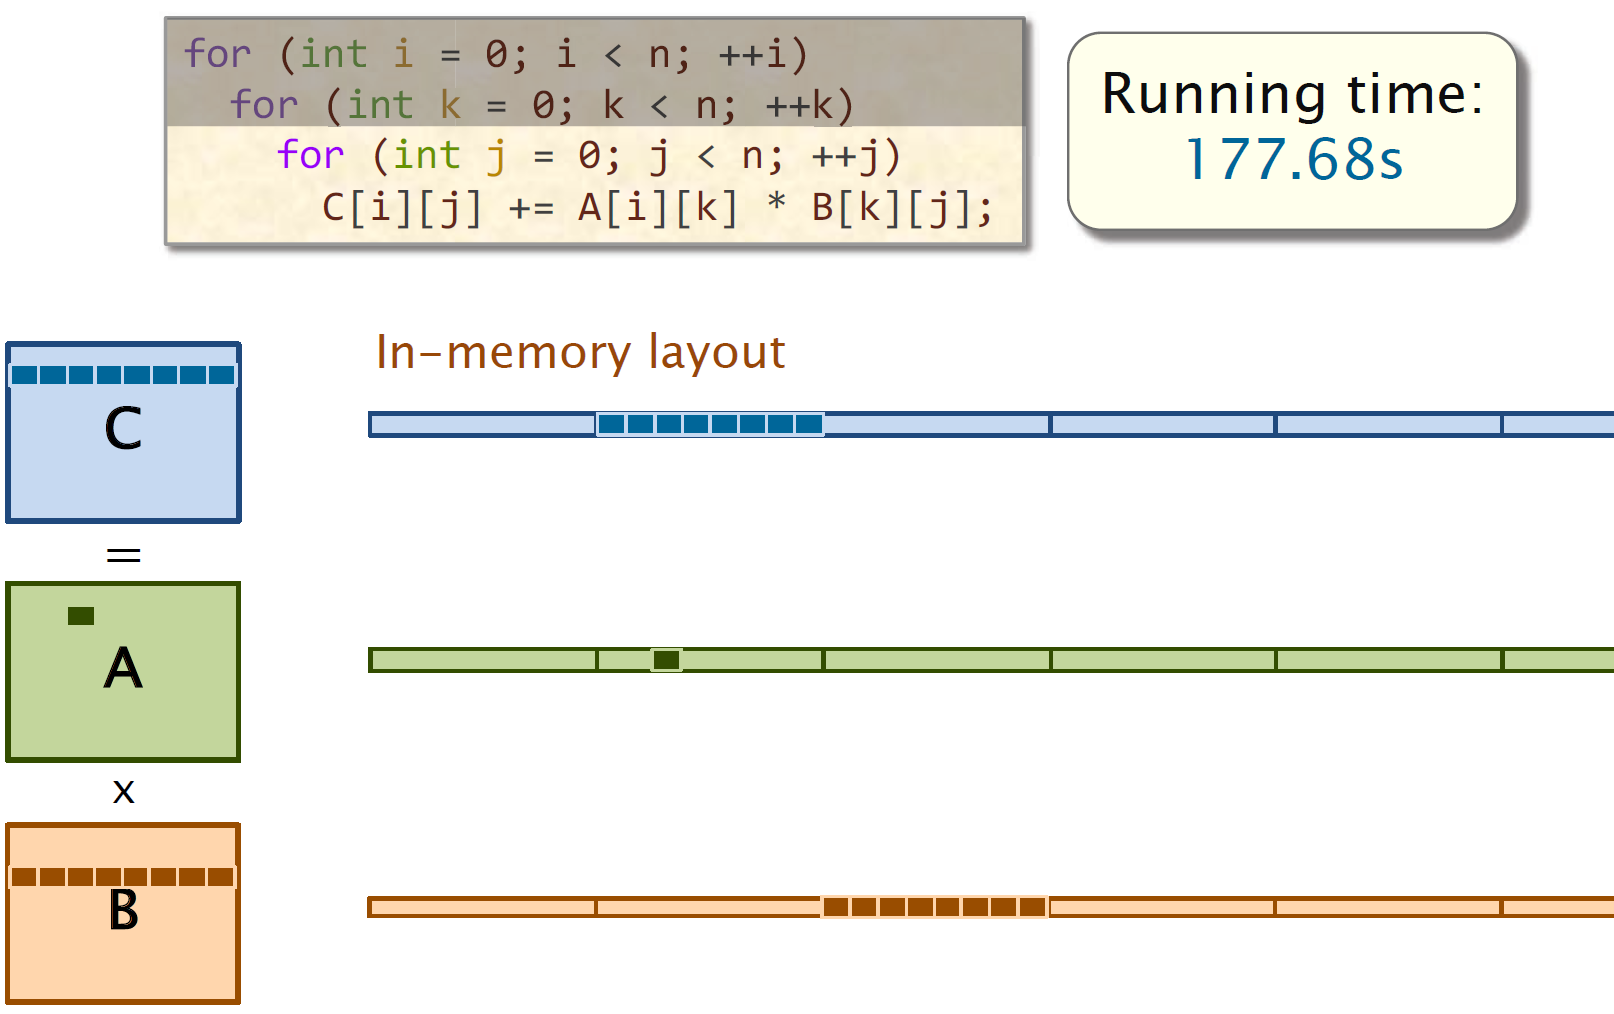
\includegraphics[width=0.49\columnwidth]{images/02/memory_layout2.png}\\
   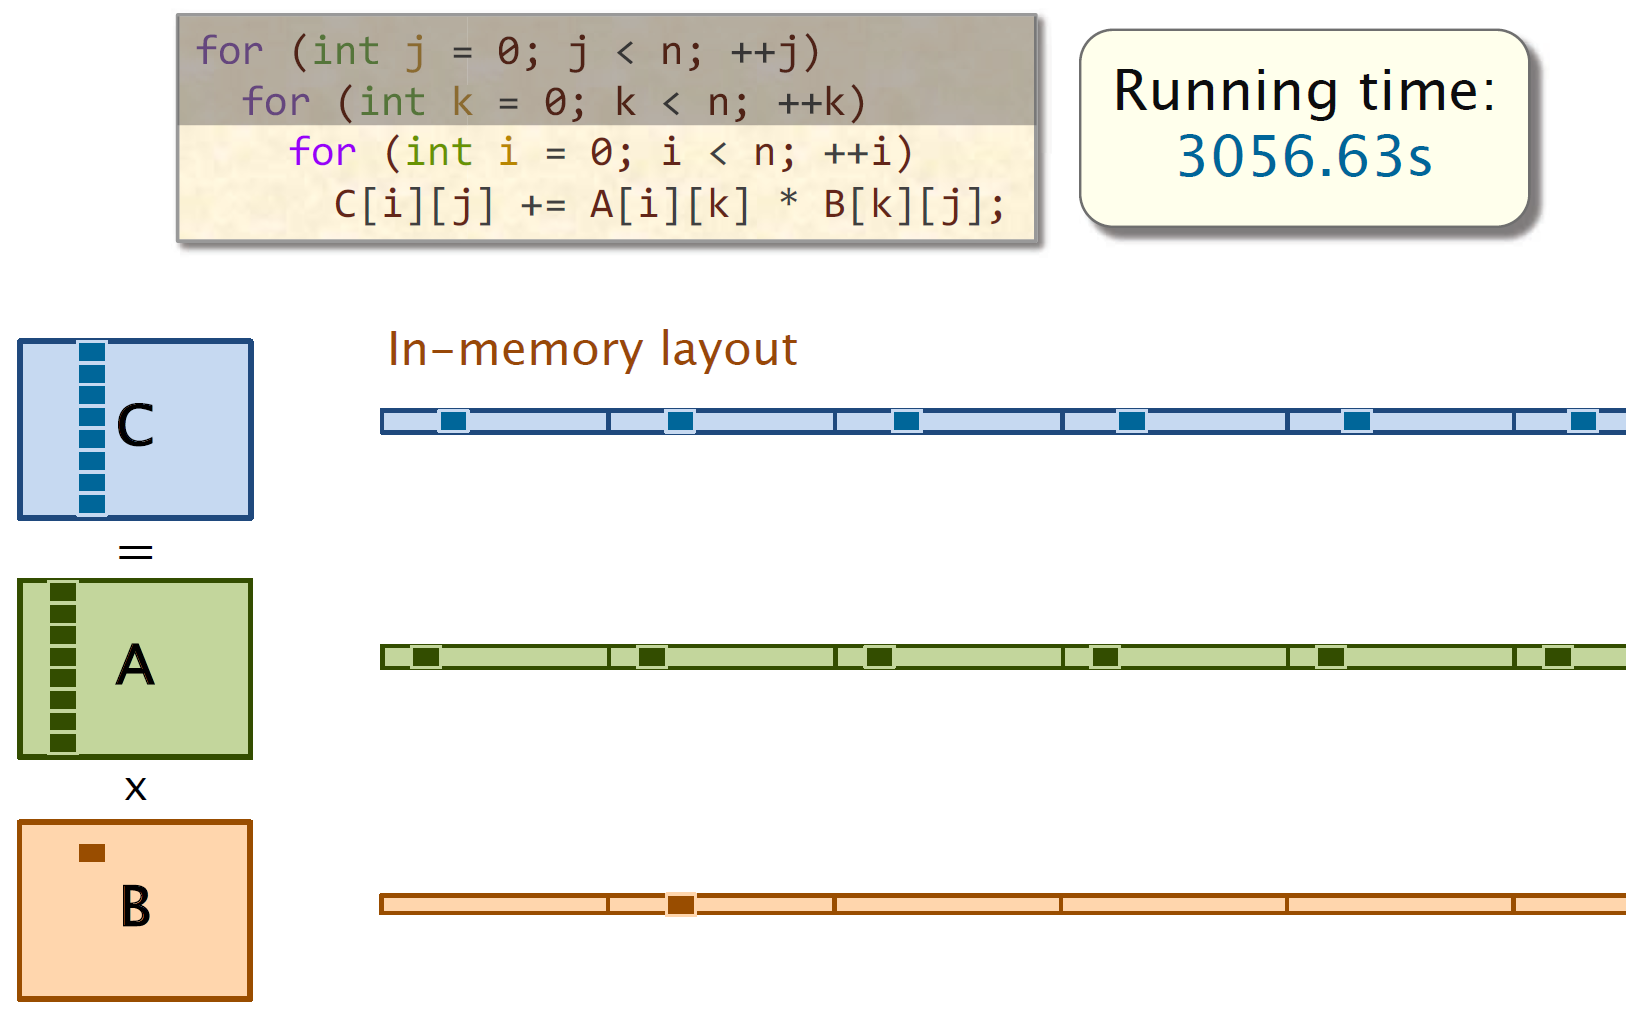
\includegraphics[width=0.49\columnwidth]{images/02/memory_layout3.png}
   \caption{Memory layout and spaciality implications}
   \label{fig:02/spaciality}
\end{figure}

\section{Compiler Optimization}
\begin{paracol}{2}
   \colfill
   Clang offers a lot of optimization flags, like \texttt{-O3} which enables all the optimizations. The compiler can also unroll loops, which means that it can execute multiple iterations of the loop in parallel. This can be done only if the number of iterations is known at compile time.
   There are also \texttt{-0s} which optimizes for size, and \texttt{-0g} which generates debug information. There's plenty of them, for various uses.
   \colfill
   
   \switchcolumn
   \begin{figure}[htbp]
      \centering
      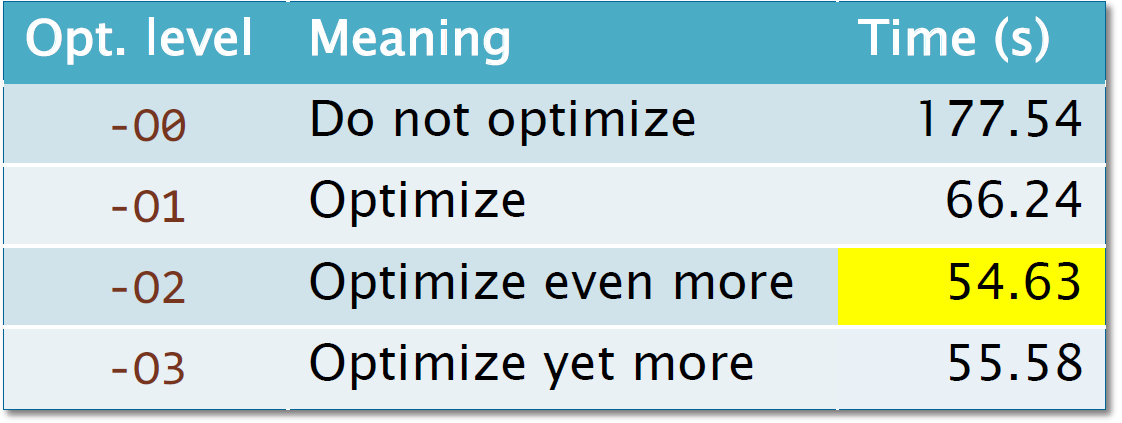
\includegraphics{images/02/optimization.png}
      \caption{Optimization flags and relative performance}
      \label{fig:02/optimization}
   \end{figure}
\end{paracol}

\section{Parallelizing}
Even after all these tweaks, we are still using only one of the 9 cores of the CPU.
So\dots
\begin{lstlisting}
   cilk_for (int i = 0; i < n; i++) {
      for (int k = 0; k < n; k++) {
         cilk_for (int j = 0; j < n; j++) {
            C[i][j] += A[i][k] +B[k][j];
         }
      }
   }
\end{lstlisting}
We don't have to know what's behind the \texttt{cilk\_for} keyword, but it will parallelize the \texttt{for} loop execution.
\framedt{
   But which \texttt{for} loops should we parallelize?
}{
   Parallelizing all three would cause multiple threads to access the same memory, which would be messy.

   A \ul{\textbf{rule of thumb} is to parallelize the \textbf{outermost} loop}, which is the one that iterates over the rows of the matrix.
   
   This is demonstrated by the following slide. 
}

\begin{figure}[htbp]
   \centering
   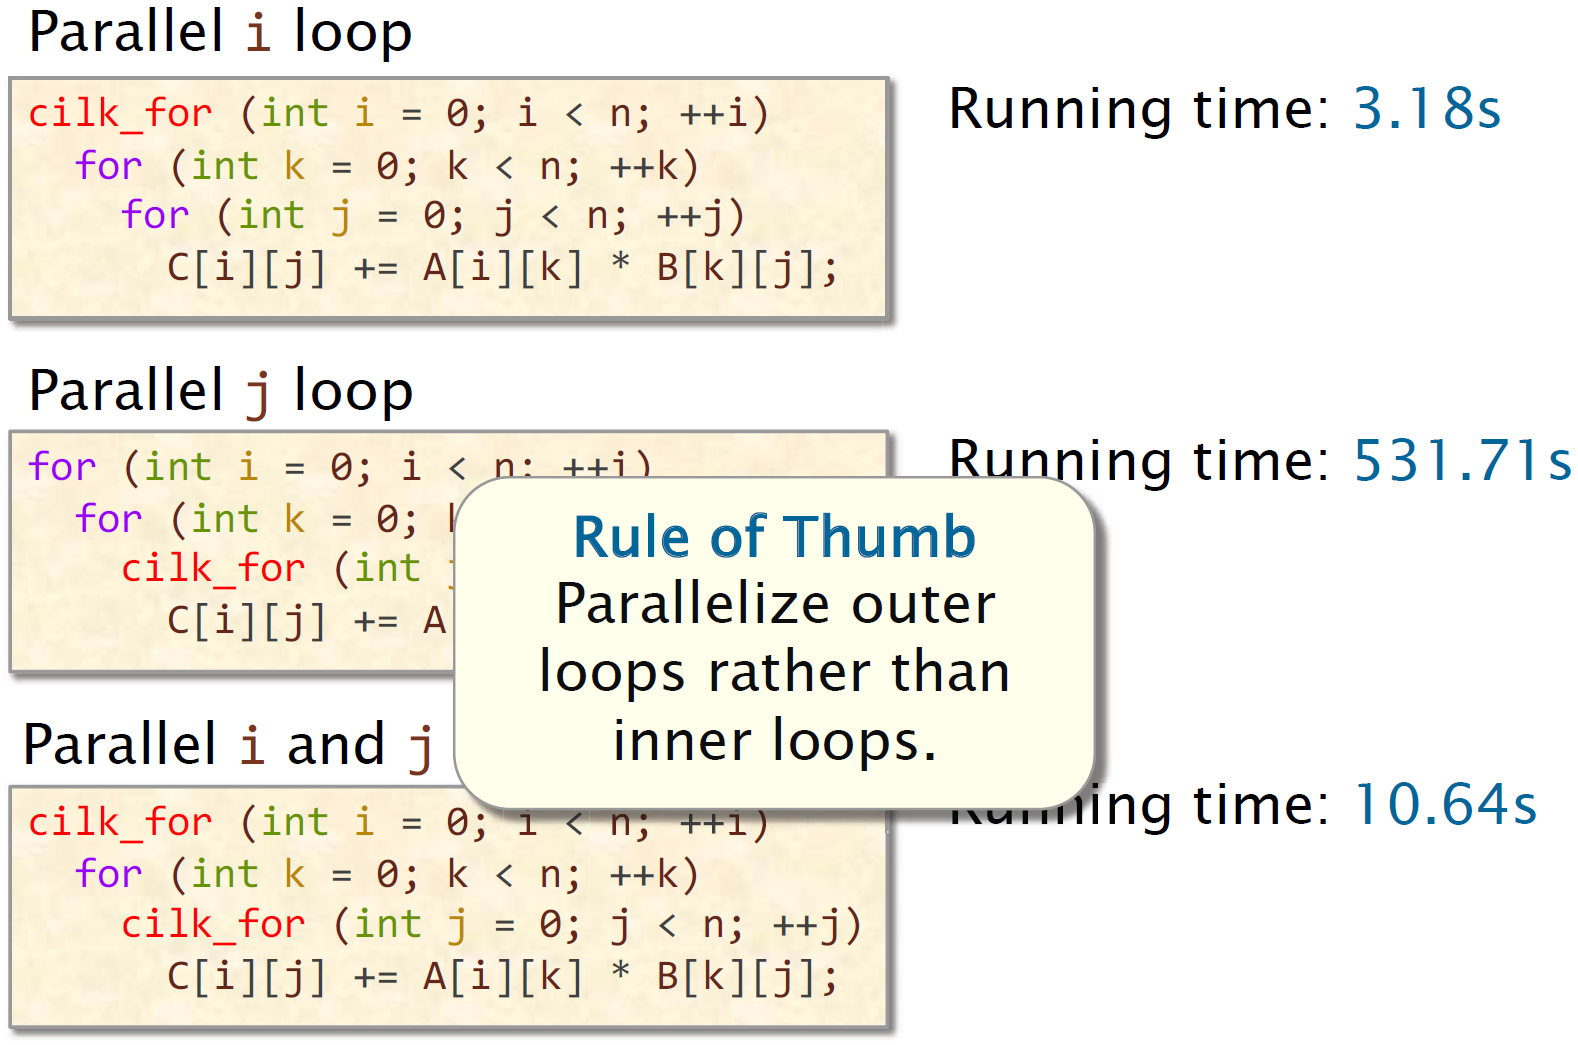
\includegraphics{images/02/loops_rule_of_thumb.png}
   \caption{Parallelizing only the outermost loop leads to optimal performance}
   \label{fig:02/loops_rule_of_thumb}
\end{figure}

\newpage
\section{Tiling}
Well, the possible optimizations ain't over \smiley.
\begin{figure}[htbp]
   \centering
   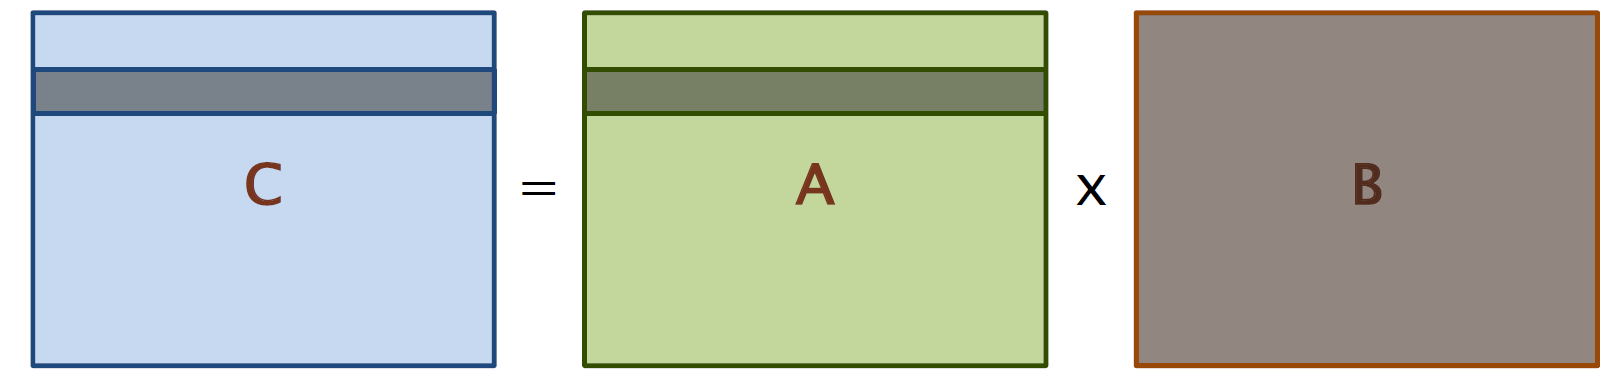
\includegraphics{images/02/tiling1.png}\\
   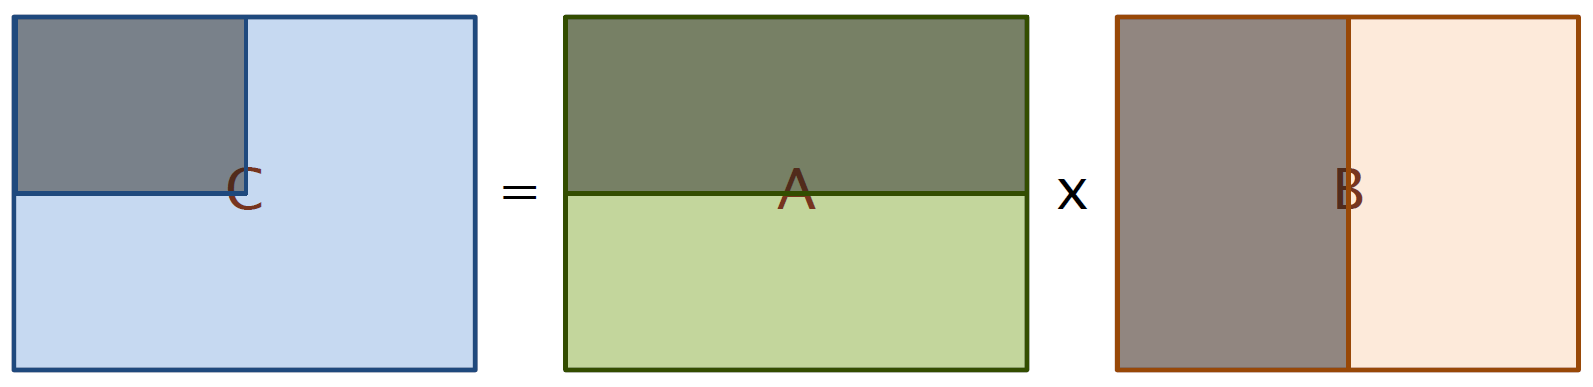
\includegraphics{images/02/tiling2.png}
   \caption{Tiling}
   \label{fig:02/tiling}
\end{figure}
Consider the first picture and let's dig into some math. How many memory accesses must the looping perform to fully compute 1 row of C? 
\begin{align}
   &4096 \cdot 1 &=\quad& 4096 \textit{ writes to C}\\
   &4096 \cdot 1 &=\quad& 4096 \textit{ reads from C}\\
   &4096 \cdot 4096 &=\quad& 1.6777216\cdot 10^6 \textit{ reads from B}\\
   &1.6777216 + 4096 + 4096 &=\quad& 1.6785408\cdot 10^6 \textit{ total memory accesses}
\end{align}

But if we consider instead computing a $64\times 64$ block of C we can shrink down the number of memory accesses to half a million:
\begin{align}
   & 64 \cdot 64 &=\quad&  4096 \textit{ writes to C}\\
   & 64 \cdot 4096 &=\quad&  262144 \textit{ reads from A}\\
   & 4096 \cdot 64 &=\quad&  262144 \textit{ reads from B}\\
   & 262144 + 262144 + 4096 &=\quad&  528384 \textit{ total memory accesses}\\
\end{align}

But in general, which would the optimal block size be? The only way is to experiment.
\note{Why?}
\begin{figure}[htbp]
   \centering
   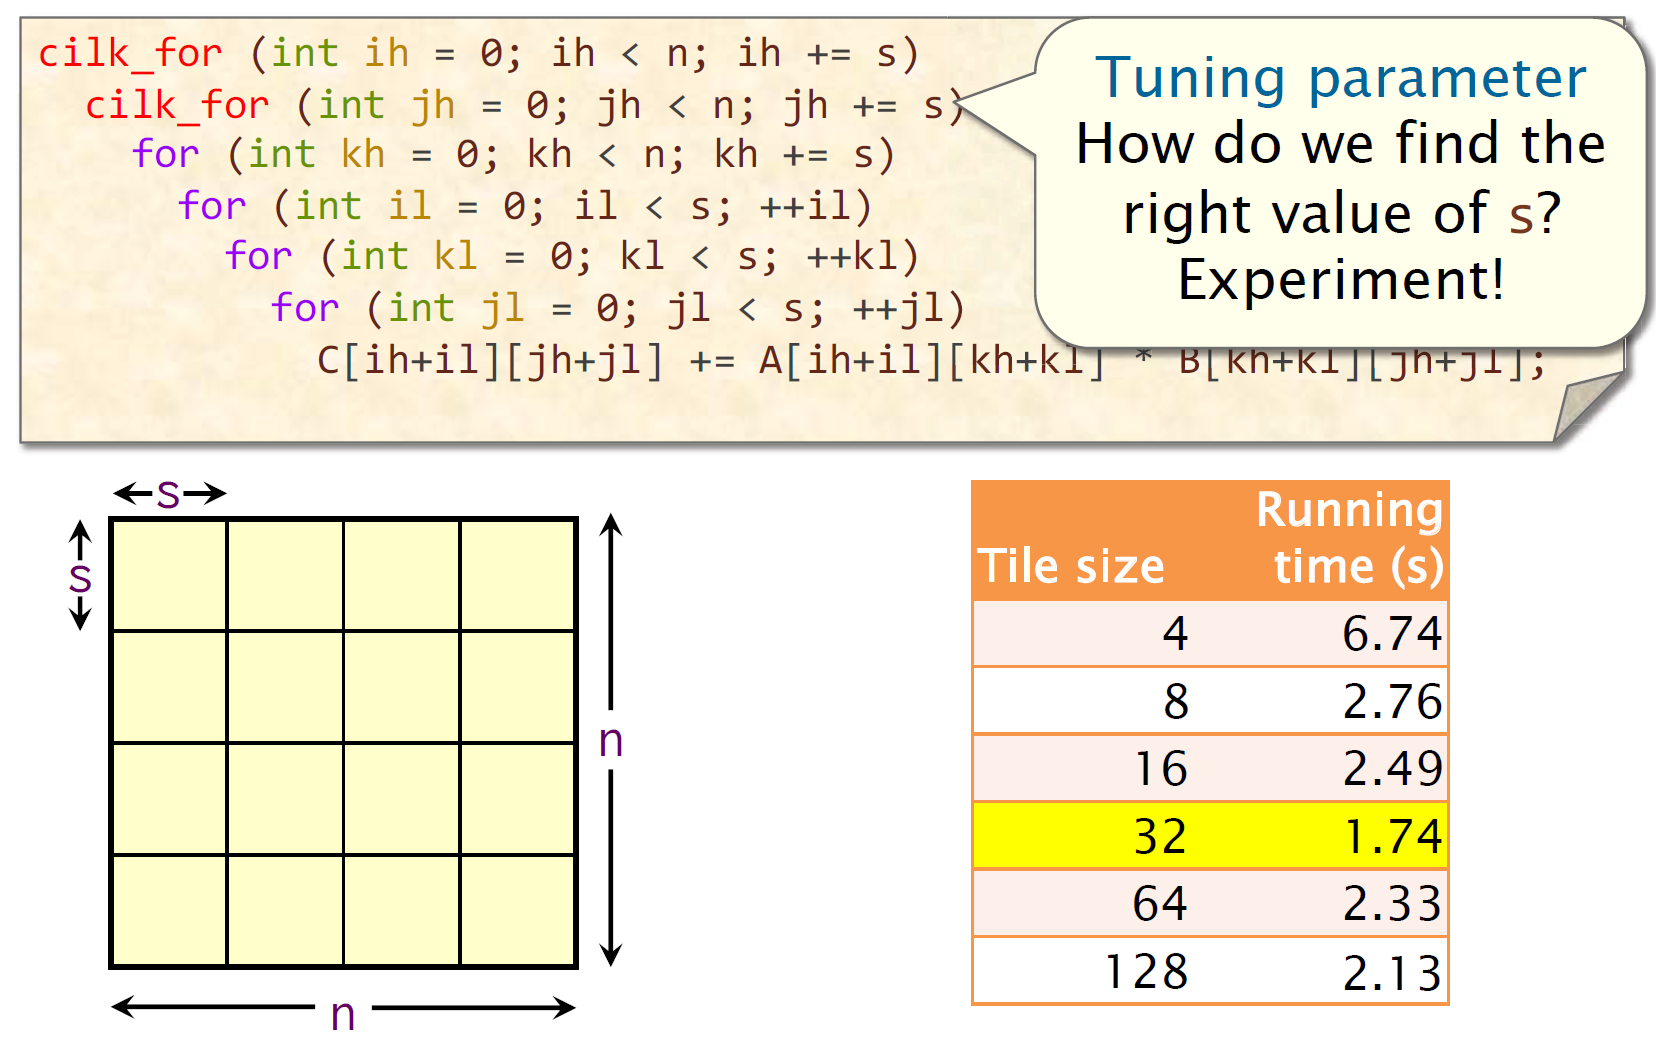
\includegraphics{images/02/tiling_size.png}
   \caption{Tile size}
   \label{fig:02/tiling_size}
\end{figure}
\newpage

\section{Where have we gotten so far - Further optimizations}
\begin{figure}[htbp]
   \centering
   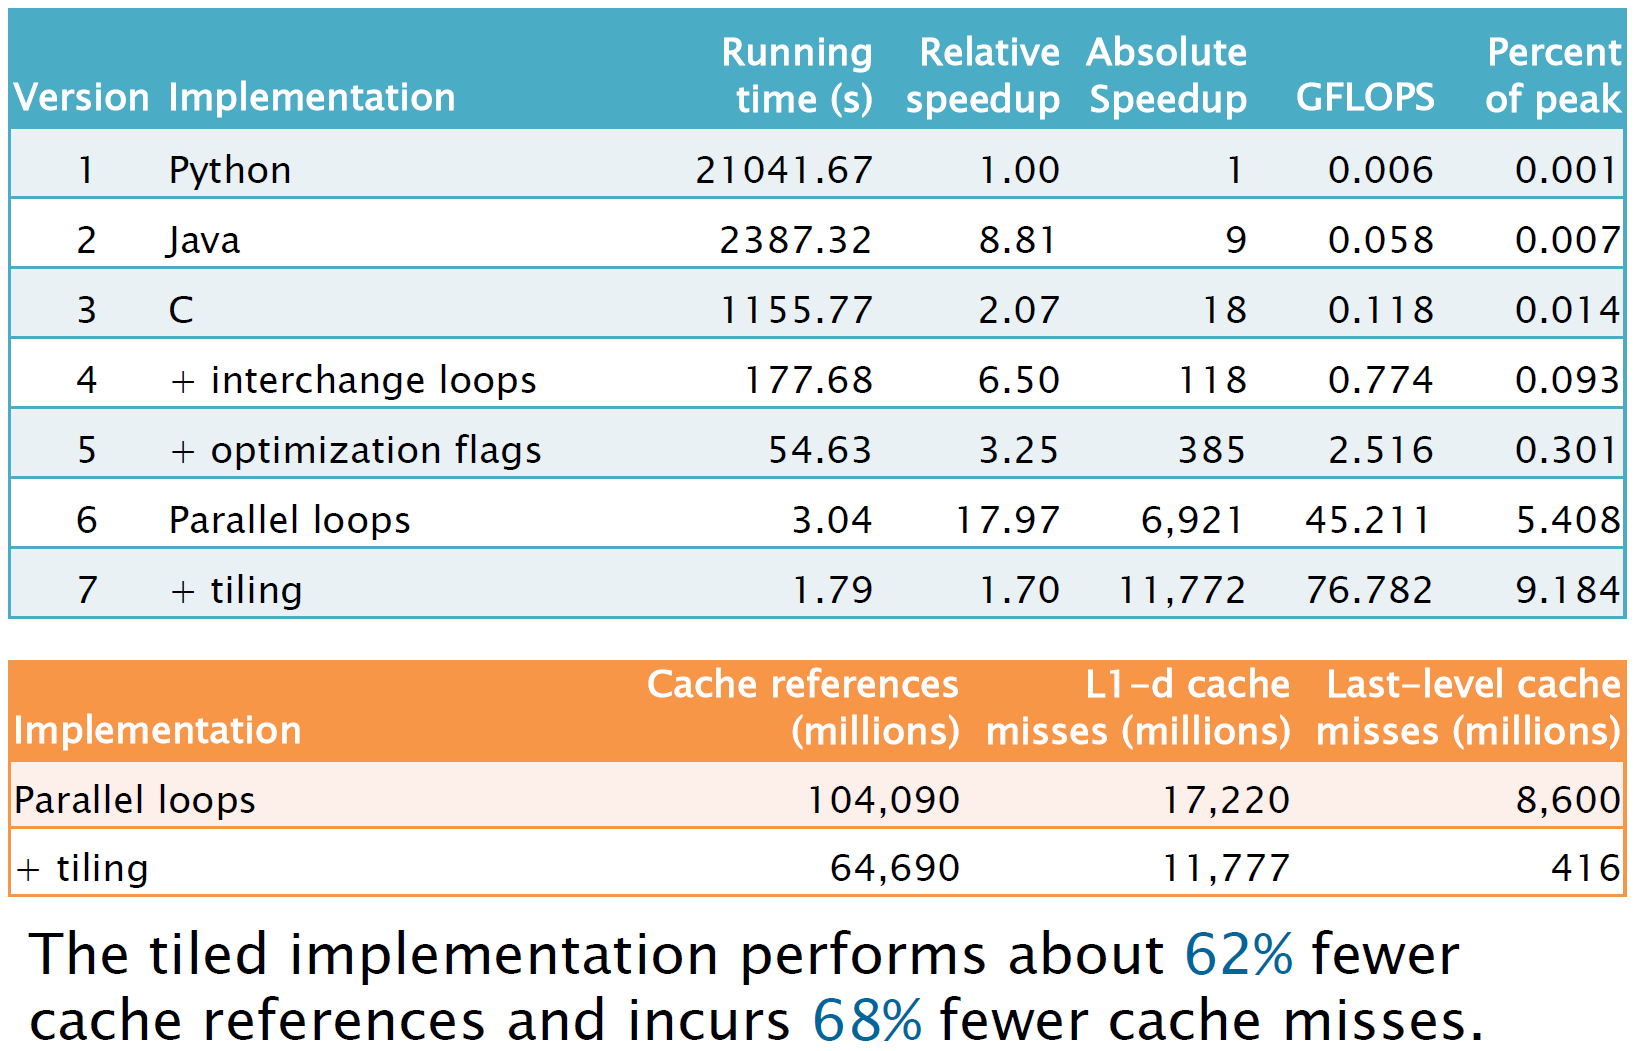
\includegraphics{images/02/comparison.png}
   \caption{Comparison of the various optimizations}
   \label{fig:02/comparison}
\end{figure}

\subsection{Recursion in Tiling}
Tiling may be also implemented as a divide-and-conquer algorithm exploiting recursion. This yields slightly better performance, but requires to tune the recursion base case \textbf{threshold}.
Having a too small threshold would lead to a lot of overhead, due to many function invocations.

\subsection{Vectorization Flags}
There may be also flags to enable instructions specific of a given architecture:
\begin{itemize}
   \item \texttt{-mavx}: Use Intel AVX vector instructions.
   \item \texttt{-mavx2}: Use Intel AVX2 vector instructions.
   \item \texttt{-mfma}: Use fused multiply-add vector instructions.
   \item \texttt{-march=<string>}: Use whatever instructions are available on the specified architecture.
   \item \texttt{-march=native}: Use whatever instructions are available on the architecture of the machine doing compilation.
   \item[] Due to restrictions on floating-point arithmetic, additional flags, such as \texttt{-ffast-math}, might be needed for these vectorization flags to have an effect
\end{itemize}

You could also use \texttt{AVX Intrinsic Instructions} that provide access to hardware vector operations. They are available in C and C++.
\href{https://software.intel.com/sites/landingpage/IntrinsicsGuide/}{software.intel.com/sites/landingpage/IntrinsicsGuide}.\\
These may help further more, but we are getting very closer to the hardware.